\mysection{Статистика количества аргументов функций}
\label{args_stat}

Всегда было интересно узнать, какое среднее количество аргументов у ф-ций.

\myindex{UNIX!grep}
Я проанализировал множетсво DLL из 32-битной Windows 7 \\
(crypt32.dll, mfc71.dll, msvcr100.dll, shell32.dll, 
user32.dll, d3d11.dll, mshtml.dll, msxml6.dll, sqlncli11.dll, wininet.dll, mfc120.dll, msvbvm60.dll, ole32.dll, themeui.dll, wmp.dll) 
(потому что они используют соглашение о вызовах \emph{stdcall}, так что легко просто \emph{grep-ать} вывод дизассемблера используя
просто \INS{RETN X}).

\begin{itemize}
\item без аргументов: $\approx 29\%$
\item 1 аргумент: $\approx 23\%$
\item 2 аргументов: $\approx 20\%$
\item 3 аргументов: $\approx 11\%$
\item 4 аргументов: $\approx 7\%$
\item 5 аргументов: $\approx 3\%$
\item 6 аргументов: $\approx 2\%$
\item 7 аргументов: $\approx 1\%$
\end{itemize}

\begin{figure}[H]
\centering
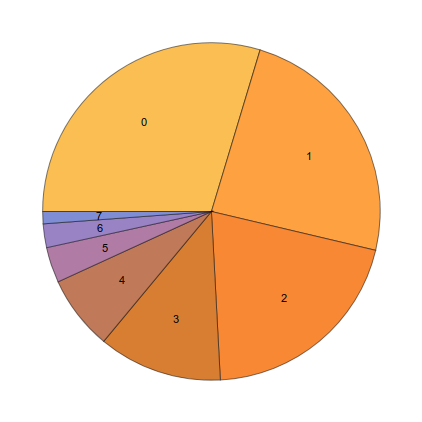
\includegraphics[width=0.5\textwidth]{other/args_stat.png}
\caption{Статистика количества аргументов функций}
\end{figure}

Это сильно зависит от стиля программирования, и может быть совсем другим в другом ПО.

